\section{CUDA/OpenACC interoperability}

\begin{frame}
	\frametitle{Why bother???}
	\begin{columns}
		\column{0.5\textwidth}
		\begin{itemize}
			\item OpenACC IS powerful, but has limitations...
			\item Many external libraries are CUDA-based
			\item CUDA can be overkill for simple tasks
			\item Many spatial discretizations can be efficiently implemented with OpenACC!
			\item Even in Fortran, interoperability is quite simple!
		\end{itemize}
		\column{0.5\textwidth}
		\begin{figure}
			\centering
			
\includegraphics[width=0.8\textwidth]{images/NVIDIACuda_Logo.jpg}
			
\includegraphics[width=0.8\textwidth]{images/OpenACC-logo.png}
		\end{figure}

	\end{columns}
\end{frame}

\begin{frame}
	\frametitle{Building interoperable code}
	\begin{columns}
		\column{0.5\textwidth}
		\begin{itemize}
			\item Requirements: CUDA Toolkit + OpenACC-capable compiler
			\item CUDA + C++: keep separate files and cross-compile
			\item CUDA + Fortran: NVFORTRAN can compile both, same source!
			\item CMake is your friend!
			\item Examples include a minimal CMake infra for CUDA Fortran
			\item For C/C++: declare both CUDA and C/C++ languages in your \textbf{project(...)} command, use \textbf{.cu} extension for CUDA files
		\end{itemize}
		\column{0.5\textwidth}
		\begin{figure}
			\centering
			
\includegraphics[width=0.8\textwidth]{images/cmake-logo.png}
		\end{figure}
		\begin{alertblock}{Note}
			\begin{itemize}
				\item NVC/NVC++ CAN handle CUDA commands and kernels, but NVCC is the RECOMMENDED CUDA compiler!
				\item Check the \textbf{nvidia-smi} tool for your GPU architecture
				\item CMake  can be used to bake in this functionality
			\end{itemize}
		\end{alertblock}
	\end{columns}
\end{frame}

\begin{frame}
	\frametitle{Examples/exercises}
	\begin{columns}
		\column{0.5\textwidth}
		\begin{itemize}
			\item Path: \texttt{Lucas/cuda\_acc\_interop}
			\item All examples in \texttt{src} directory
			\item Building on MN5:
			\begin{itemize}
				\item \texttt{module load ...}
				\item \texttt{mkdir build; cd build}
				\item \texttt{cmake ..}
				\item \texttt{make}
			\end{itemize}
			\item This builds every example
			\item Check the root \texttt{CMakeLists.txt} for GPU architecture!!!
		\end{itemize}
		\column{0.5\textwidth}
		\begin{figure}
			\centering
			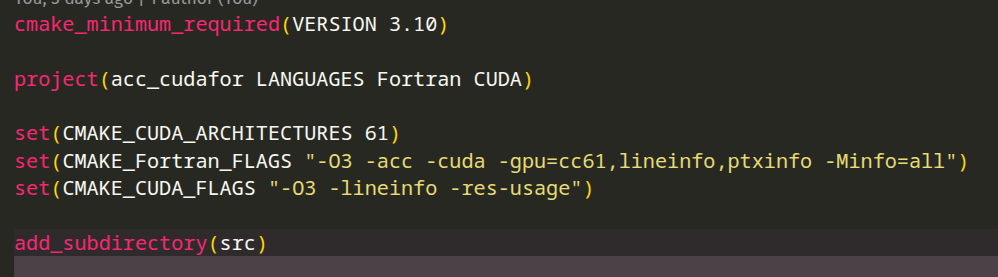
\includegraphics[width=0.99\textwidth]{images/cmakelists_1.png}
		\end{figure}
	\end{columns}
\end{frame}

\begin{frame}
	\frametitle{Example 1: ACC to CUDA}
	\begin{columns}
		\column{0.5\textwidth}
		\begin{itemize}
			\item ACC: manage device data creation and movement
			\item CUDA: define executable kernels
			\item Key detail: use of \texttt{acc host\_data use\_device} block wrapping kernel calls
			\item After update and print, another CUDA kernel is called to demonstrate that data is still on device, and usable!
			\item cuBLAS call demonstrates interoperability with CUDA libraries
			\item Exercise: run with NSYS tool to check data movements and kernel calls
		\end{itemize}
		\column{0.5\textwidth}
		\begin{figure}
			\centering
			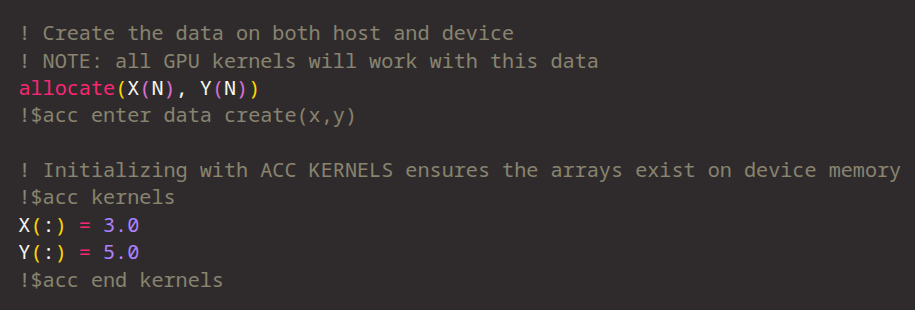
\includegraphics[width=0.9\textwidth]{images/acc2cuda_data.png}
			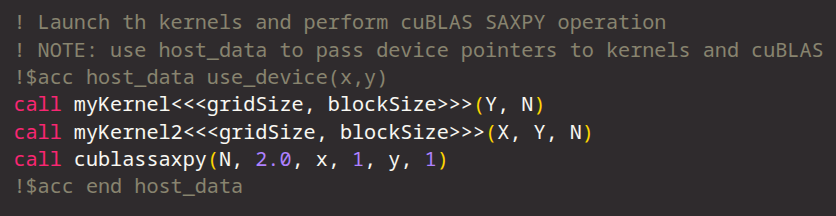
\includegraphics[width=0.9\textwidth]{images/acc2cuda_kernels.png}
		\end{figure}
	\end{columns}
\end{frame}

\begin{frame}
	\frametitle{Example 2: CUDA to ACC}
	\begin{columns}
		\column{0.5\textwidth}
		\begin{itemize}
			\item CUDA: handle device data creation and movement
			\item ACC: GPU kernels
			\item Key detail: CUDA Fortran arrays declared with \texttt{device} attribute are allocated on device (mask for \texttt{cudaMalloc})
			\item The fortran assignment operator (=) is overloaded to perform host/device copies (mask for \texttt{cudaMemcpy})
			\item ACC kernels include a subroutine call to demonstrate how a CUDA Fortran device array can be passed to an extrnal ACC kernel
			\item Exercise: run with NSYS tool to check data movements and kernel calls
		\end{itemize}
		\column{0.5\textwidth}
		\begin{figure}
			\centering
			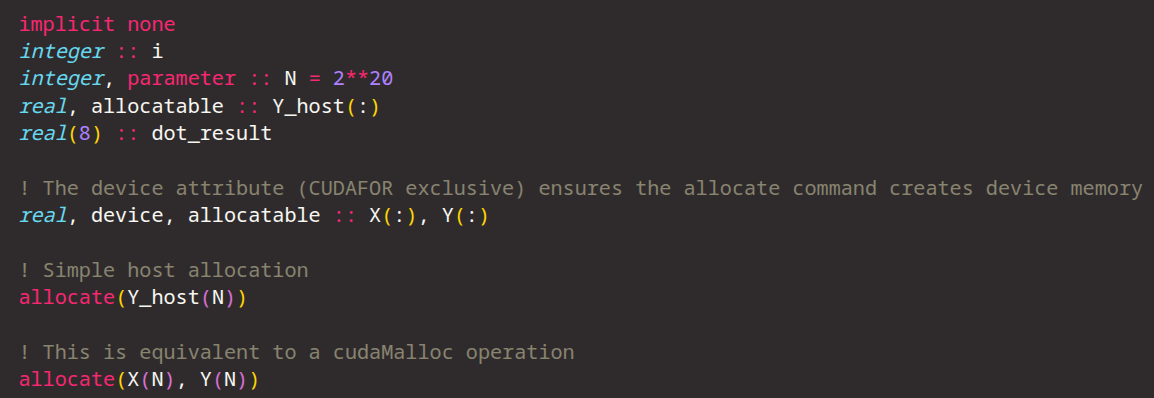
\includegraphics[width=0.9\textwidth]{images/cuda2acc_data.png}
			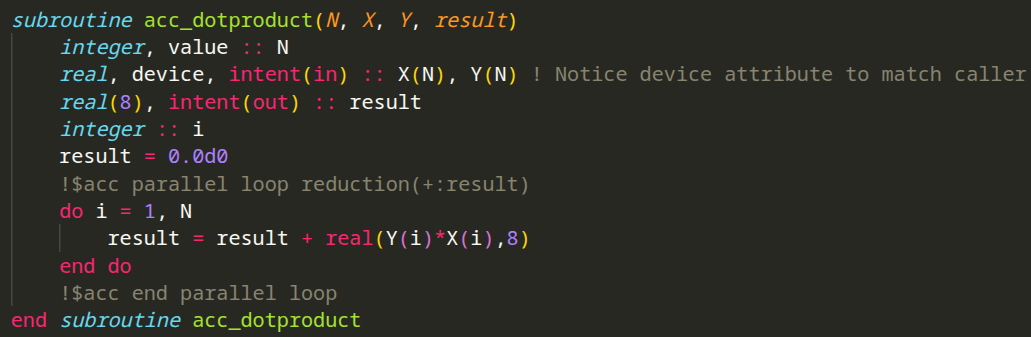
\includegraphics[width=0.9\textwidth]{images/cuda2acc_routine.png}
		\end{figure}
	\end{columns}
\end{frame}